\section{Exploratory Data Analysis (EDA)}

\subsection{Target Class Distribution}
The first step in our analysis is to check the balance of our target variable.

\begin{figure}[H]
	\centering
	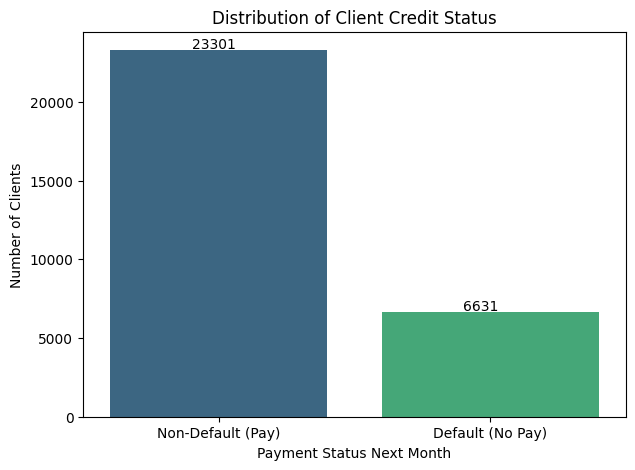
\includegraphics[width=0.82\textwidth]{image1.png}
	\caption{Distribution of Client Credit Status}
\end{figure}

\textbf{Interpretation:}
The dataset exhibits a significant class imbalance, with approximately 22.1\% of clients falling into the "Default" category. This imbalance indicates that accuracy alone will not be a reliable metric for model performance. We must prioritize Recall and F1-Score to ensure the model effectively identifies potential defaulters.

\subsection{Age Distribution vs. Default Status}
We examine how the age of a client correlates with their likelihood of defaulting on payments.

\begin{figure}[H]
	\centering
	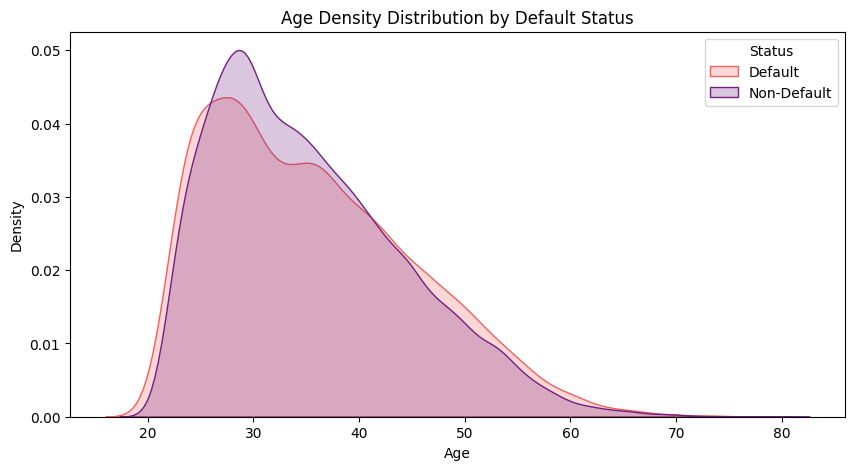
\includegraphics[width=0.82\textwidth]{image2.png}
	\caption{Age Density Distribution by Default Status}
\end{figure}

\textbf{Interpretation:}
The density plot shows that younger clients, specifically those between 20 and 30 years old, have a higher relative density of defaults. As clients age beyond 40, the probability of default tends to stabilize and decrease. This suggests that Age is a relevant demographic feature for credit risk assessment.

\subsection{Repayment Behavior (PAY\_0) Analysis}
This plot explores the relationship between the most recent repayment status and the probability of default.

\begin{figure}[H]
	\centering
	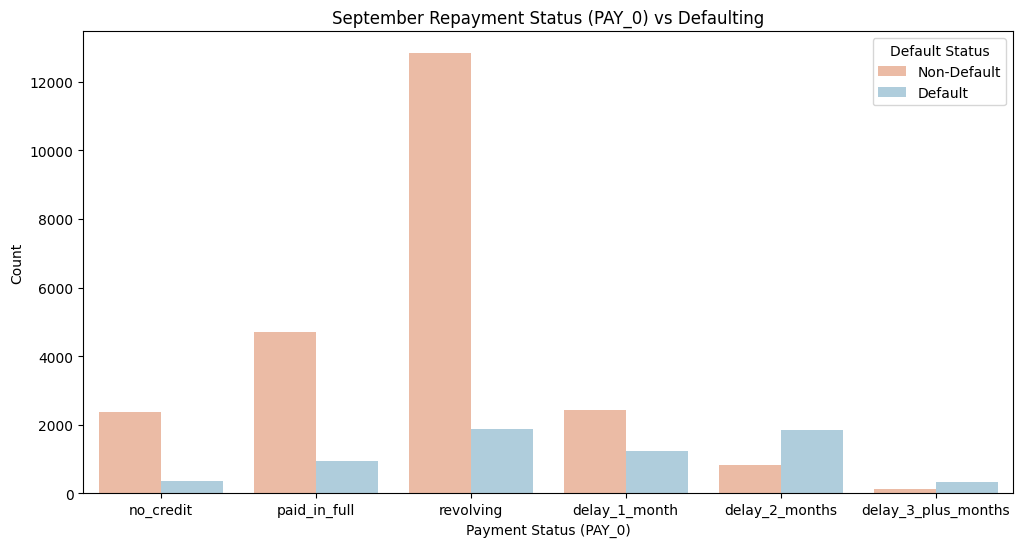
\includegraphics[width=0.82\textwidth]{image3.png}
	\caption{September Repayment Status (PAY\_0) vs Defaulting}
\end{figure}

\textbf{Interpretation:}
Clients with a PAY\_0 value of 2 or higher (representing a 2-month delay or more) show a much higher ratio of defaults. A status of 0 or -1 (on-time or early payment) strongly correlates with successful repayment next month. Behavioral history, particularly recent delays, appears to be the strongest predictor in this dataset.

\subsection{Feature Correlation Heatmap}
Finally, we analyze the correlations between numerical features to identify multicollinearity.

\begin{figure}[H]
	\centering
	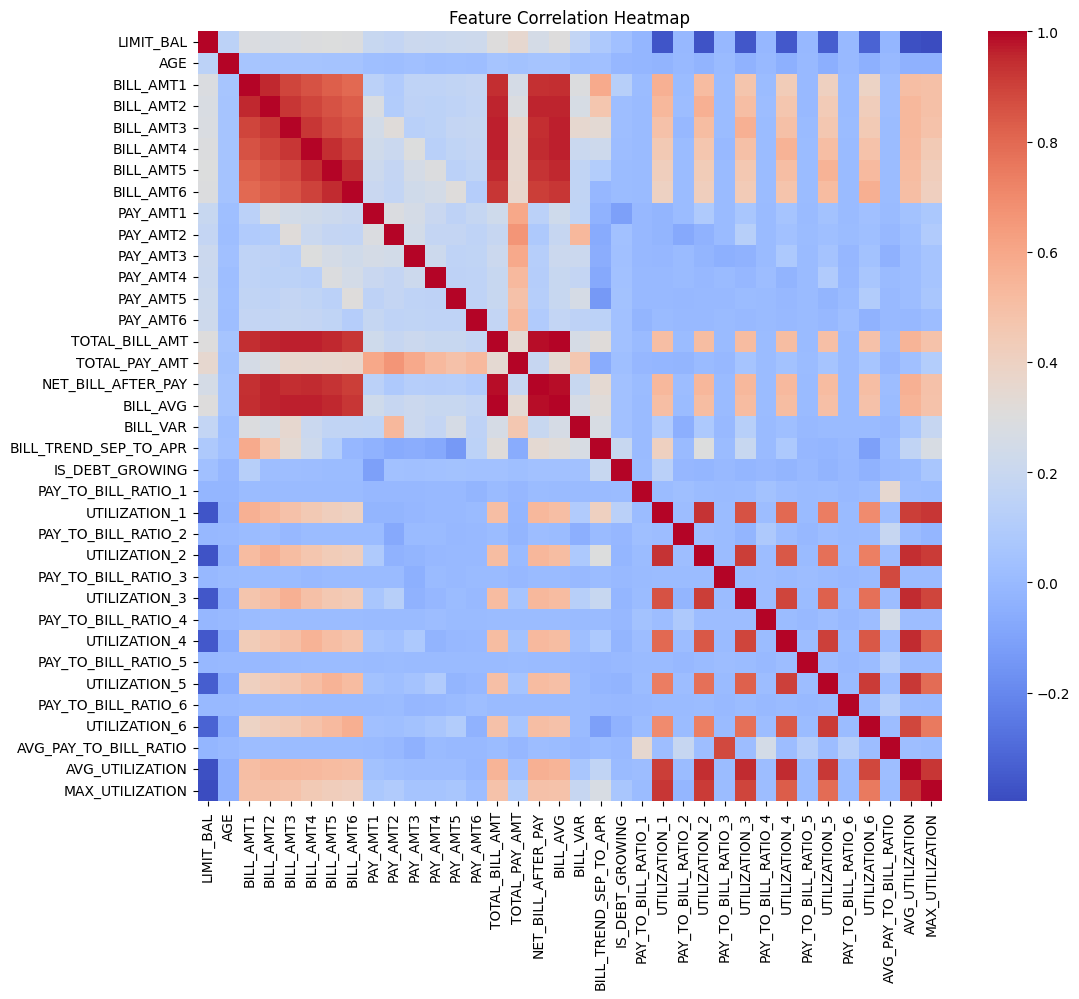
\includegraphics[width=0.9\textwidth]{image4.png}
	\caption{Feature Correlation Heatmap}
\end{figure}

High positive correlation (approaching 1.0) is observed among the BILL\_AMT and UTILIZATION feature groups. This redundancy justifies the removal of several columns to prevent overfitting and improve model stability. Features such as PAY\_0 and LIMIT\_BAL show distinct correlation patterns with the target, confirming their predictive importance.
